% Arquivo LaTeX de exemplo de dissertação/tese a ser apresentados à CPG do IME-USP
%
% Versão 5: Sex Mar  9 18:05:40 BRT 2012
%
% Criação: Jesús P. Mena-Chalco
% Revisão: Fabio Kon e Paulo Feofiloff
%
% Obs: Leia previamente o texto do arquivo README.txt

\documentclass[12pt,twoside,a4paper]{book}

% ---------------------------------------------------------------------------- %
% Pacotes
\usepackage[utf8]{inputenc}
\usepackage[T1]{fontenc}
\usepackage[english]{babel}
\usepackage[pdftex]{graphicx}           % usamos arquivos pdf/png como figuras
\usepackage{setspace}                   % espaçamento flexível
\usepackage{indentfirst}                % indentação do primeiro parágrafo
\usepackage{makeidx}                    % índice remissivo
\usepackage[nottoc]{tocbibind}          % acrescentamos a bibliografia/indice/conteudo no Table of Contents
\usepackage{sourcecodepro}
\usepackage{type1cm}                    % fontes realmente escaláveis
\usepackage{listings}                   % para formatar código-fonte (ex. em Java)
\usepackage{titletoc}
\usepackage{booktabs}
\usepackage{textcomp}
\usepackage[explicit]{titlesec} % cabeçalhos dos títulos: menores e compactos
\usepackage{tocloft}
\usepackage{amssymb}
\usepackage{epigraph}
\usepackage[fixlanguage]{babelbib}
\usepackage[font=small,format=plain,labelfont=bf,up,textfont=it,up]{caption}
\usepackage[usenames,svgnames,dvipsnames]{xcolor}
\usepackage{wrapfig}
\usepackage[a4paper,top=2.54cm,bottom=2.0cm,left=2.0cm,right=2.54cm]{geometry} % margens
%\usepackage[pdftex,plainpages=false,pdfpagelabels,pagebackref,colorlinks=true,citecolor=black,linkcolor=black,urlcolor=black,filecolor=black,bookmarksopen=true]{hyperref} % links em preto
\usepackage[pdftex,plainpages=false,pdfpagelabels,pagebackref,colorlinks=true,citecolor=DarkGreen,linkcolor=NavyBlue,urlcolor=DarkRed,filecolor=green,bookmarksopen=true]{hyperref} % links coloridos
\usepackage[all]{hypcap}                    % soluciona o problema com o hyperref e capitulos
\usepackage[round,sort,nonamebreak,numbers]{natbib} % citação bibliográfica textual(plainnat-ime.bst)
%\fontsize{60}{62}\usefont{OT1}{cmr}{m}{n}{\selectfont}
\setlength{\epigraphrule}{0pt}
\setlength{\epigraphwidth}{8cm}
\renewcommand{\textflush}{flushepinormal}

% ---------------------------------------------------------------------------- %
% Cabeçalhos similares ao TAOCP de Donald E. Knuth
\usepackage{fancyhdr}
\pagestyle{fancy}
\fancyhf{}
\renewcommand{\chaptermark}[1]{\markboth{#1}{}}
\renewcommand{\sectionmark}[1]{\markright{#1}}
\renewcommand{\headrulewidth}{0pt}

\fancyhead[LE,RO]{\thepage}
\fancyhead[LO]{\itshape\nouppercase{\rightmark}}
\fancyhead[RE]{\itshape\nouppercase{\leftmark}}

% ---------------------------------------------------------------------------- %
\graphicspath{{./images/}}             % caminho das figuras (recomendável)
\frenchspacing                          % arruma o espaço: id est (i.e.) e exempli gratia (e.g.)
\urlstyle{same}                         % URL com o mesmo estilo do texto e não mono-spaced
\makeindex                              % para o índice remissivo
\raggedbottom                           % para não permitir espaços extra no texto
%\fontsize{60}{62}\usefont{OT1}{cmr}{m}{n}{\selectfont}
\cleardoublepage
\normalsize

% ---------------------------------------------------------------------------- %
% Opções de listing usados para o código fonte
% Ref: http://en.wikibooks.org/wiki/LaTeX/Packages/Listings
\lstset{ %
language=Java,                  % choose the language of the code
basicstyle=\footnotesize,       % the size of the fonts that are used for the code
numbers=left,                   % where to put the line-numbers
numberstyle=\footnotesize,      % the size of the fonts that are used for the line-numbers
stepnumber=1,                   % the step between two line-numbers. If it's 1 each line will be numbered
numbersep=5pt,                  % how far the line-numbers are from the code
showspaces=false,               % show spaces adding particular underscores
showstringspaces=false,         % underline spaces within strings
showtabs=false,                 % show tabs within strings adding particular underscores
frame=single,                    % adds a frame around the code
framerule=0.6pt,
tabsize=2,                        % sets default tabsize to 2 spaces
captionpos=b,                   % sets the caption-position to bottom
breaklines=true,                % sets automatic line breaking
breakatwhitespace=false,        % sets if automatic breaks should only happen at whitespace
escapeinside={\%*}{*)},         % if you want to add a comment within your code
backgroundcolor=\color[rgb]{1.0,1.0,1.0}, % choose the background color.
rulecolor=\color[rgb]{0.8,0.8,0.8},
extendedchars=true,
xleftmargin=10pt,
xrightmargin=10pt,
framexleftmargin=10pt,
framexrightmargin=10pt
}

% Setting Chapter Style
\makeatletter
\def\thickhrulefill{\leavevmode \leaders \hrule height .1ex \hfill \kern \z@}
\def\@makechapterhead#1{%
  %\vspace*{50\p@}%
  %\vspace*{5\p@}%
  {\parindent \z@ \centering \reset@font
        \thickhrulefill\quad
        \itshape \bfseries \normalsize \@chapapp{} \thechapter
        \normalsize \quad \thickhrulefill
        \par\nobreak
        \vspace*{5\p@}%
        \interlinepenalty\@M
        %\hrule
        %\vspace*{10\p@}%
        \normalfont \LARGE \bfseries #1\par\nobreak
        \par
        \vspace*{5\p@}%
        %\hrule
    %\vskip 40\p@
    \vskip 30\p@
  }}
\def\@makeschapterhead#1{%
  %\vspace*{50\p@}%
  %\vspace*{5\p@}%
  {\parindent \z@ \centering \reset@font
        \thickhrulefill
        \par\nobreak
        \vspace*{5\p@}%
        \interlinepenalty\@M
        %\hrule
        %\vspace*{10\p@}%
        \LARGE \bfseries #1\par\nobreak
        \par
        \vspace*{5\p@}%
        %\hrule
    %\vskip 40\p@
    \vskip 30\p@
  }}

\renewcommand\cftloftitlefont{\itshape\bfseries\Large}

\renewcommand\cftlottitlefont{\itshape\bfseries\Large}

\renewcommand\cfttoctitlefont{\hfill\itshape\bfseries\Large}

\renewcommand{\cftaftertoctitle}{\hfill}

 \titleformat{\section}
  {\itshape\large\bfseries}{\thesection}{1em}{#1}

\titleformat{\subsection}
  {\itshape\normalsize\bfseries}{\thesubsection}{1em}{#1}

\titleformat{\subsubsection}
  {\normalsize\bfseries\itshape}{\thesubsubsection}{1em}{#1}

% Setting custom lists
\newcommand{\listabbreviationname}{\itshape \Large List of Abbreviations}

\newlistof{abbreviation}{abb}{\listabbreviationname}

\newcommand{\abbreviation}[2]{%
\refstepcounter{abbreviation}
%\par\noindent\textbf{Example \theexample. #1}
\addcontentsline{abb}{abbreviation}
{\protect\makebox[2cm]{#1} #2}\par}

\cftpagenumbersoff{abbreviation}

% Setting custom lists
\newcommand{\listsymbolentryname}{\itshape \Large List of Symbols}

\newlistof{symbolentry}{synt}{\listsymbolentryname}

\newcommand{\symbolentry}[2]{%
\refstepcounter{symbolentry}
%\par\noindent\textbf{Example \theexample. #1}
\addcontentsline{synt}{symbolentry}
{\protect\makebox[2cm]{#1} #2}\par}

\cftpagenumbersoff{symbolentry}

\setcitestyle{square}

% ---------------------------------------------------------------------------- %
% Corpo do texto
\begin{document}
\frontmatter
% cabeçalho para as páginas das seções anteriores ao capítulo 1 (frontmatter)
%\fancyhead[RO]{{\footnotesize\rightmark}\hspace{2em}\thepage}
\setcounter{tocdepth}{2}
%\fancyhead[LE]{\thepage\hspace{2em}\footnotesize{\leftmark}}
%\fancyhead[RE,LO]{}
%\fancyhead[RO]{{\footnotesize\rightmark}\hspace{2em}\thepage}

\onehalfspacing  % espaçamento

% ---------------------------------------------------------------------------- %
% CAPA
% Nota: O título para as dissertações/teses do IME-USP devem caber em um
% orifício de 10,7cm de largura x 6,0cm de altura que há na capa fornecida pela SPG.
\thispagestyle{empty}
\begin{center}
    \vspace*{2.3cm}
    \textbf{\Large{Parallel and Distributed Autotuning \\
                   for High-Performance Computing}}\\

    \vspace*{1.2cm}
    \Large{Pedro Bruel}

    \vskip 2cm
    \textsc{
    Text submitted\\[-0.25cm]
    to the\\[-0.25cm]
    Institute de Mathematics and Statistics\\[-0.25cm]
    of the\\[-0.25cm]
    University of São Paulo\\[-0.25cm]
    for the\\[-0.25cm]
    Qualifying examination\\[-0.25cm]
    for the\\[-0.25cm]
    Doctoral Degree in\\[-0.25cm]
    Computer Science}

    \vskip 1.5cm
    Advisor: Professor Alfredo Goldman Vel Lejbman

       \vskip 1cm
    \normalsize{During the development of this work, the author was supported
    by CNPq \textnumero XXXX, Hewlett-Packard Enterprise and CAPES}

    \vskip 0.5cm
    \normalsize{São Paulo, \today}
\end{center}

% ---------------------------------------------------------------------------- %
% Página de rosto (SÓ PARA A VERSÃO DEPOSITADA - ANTES DA DEFESA)
% Resolução CoPGr 5890 (20/12/2010)
%
% IMPORTANTE:
%   Coloque um '%' em todas as linhas
%   desta página antes de compilar a versão
%   final, corrigida, do trabalho
%
%
\newpage
\thispagestyle{empty}
    \begin{center}
        \vspace*{2.3 cm}
        \textbf{\Large{Parallel and Distributed Autotuning\\
                       for High-Performance Computing}}\\
        \vspace*{2 cm}
    \end{center}

    \vskip 2cm

    \begin{flushright}
    This is the original version\\
    submitted for evaluation\\
    by Pedro Bruel
    \end{flushright}

\pagebreak


% ---------------------------------------------------------------------------- %
% Página de rosto (SÓ PARA A VERSÃO CORRIGIDA - APÓS DEFESA)
% Resolução CoPGr 5890 (20/12/2010)
%
% Nota: O título para as dissertações/teses do IME-USP devem caber em um
% orifício de 10,7cm de largura x 6,0cm de altura que há na capa fornecida pela SPG.
%
% IMPORTANTE:
%   Coloque um '%' em todas as linhas desta
%   página antes de compilar a versão do trabalho que será entregue
%   à Comissão Julgadora antes da defesa
%
%
%\newpage
%\thispagestyle{empty}
%    \begin{center}
%        \vspace*{2.3 cm}
%        \textbf{\Large{Título do trabalho a ser apresentado à \\
%        CPG para a dissertação/tese}}\\
%        \vspace*{2 cm}
%    \end{center}
%
%    \vskip 2cm
%
%    \begin{flushright}
%    Esta versão da dissertação/tese contém as correções e alterações sugeridas\\
%    pela Comissão Julgadora durante a defesa da versão original do trabalho,\\
%    realizada em xx/xx/2017. Uma cópia da versão original está disponível no\\
%    Instituto de Matemática e Estatística da Universidade de São Paulo.
%
%    \vskip 2cm
%
%    \end{flushright}
%    \vskip 4.2cm
%
%    \begin{quote}
%    \noindent Comissão Julgadora:
%
%    \begin{itemize}
%        \item Profª. Drª. Nome Completo (orientadora) - IME-USP [sem ponto final]
%        \item Prof. Dr. Nome Completo - IME-USP [sem ponto final]
%        \item Prof. Dr. Nome Completo - IMPA [sem ponto final]
%    \end{itemize}
%
%    \end{quote}
%\pagebreak


\pagenumbering{roman}     % começamos a numerar

% ---------------------------------------------------------------------------- %
% Agradecimentos:
% Se o candidato não quer fazer agradecimentos, deve simplesmente eliminar esta página
%\chapter*{Agradecimentos}
%Texto texto texto texto texto texto texto texto texto texto texto texto texto
%texto texto texto texto texto texto texto texto texto texto texto texto texto
%texto texto texto texto texto texto texto texto texto texto texto texto texto
%texto texto texto texto. Texto opcional.


% ---------------------------------------------------------------------------- %
% Resumo
%\chapter*{Resumo}
%
%\noindent BRUEL, P. \textbf{Título do trabalho em português}.
%2017. xxx f.
%Qualificação (Doutorado) - Instituto de Matemática e Estatística,
%Universidade de São Paulo, São Paulo, 2010.
%\\
%
%Elemento obrigatório, constituído de uma sequência de frases concisas e
%objetivas, em forma de texto.  Deve apresentar os objetivos, métodos empregados,
%resultados e conclusões.  O resumo deve ser redigido em parágrafo único, conter
%no máximo 500 palavras e ser seguido dos termos representativos do conteúdo do
%trabalho (palavras-chave).
%\\
%
%\noindent \textbf{Palavras-chave:} palavra-chave1, palavra-chave2, palavra-chave3.
%
%\vspace*{1cm}%
%\thickhrulefill

% ---------------------------------------------------------------------------- %
% Abstract
\chapter*{Abstract}
\noindent BRUEL, P. \textbf{Parallel and Distributed Autotuning for High-Performance Computing}.
2017. xxx f.
Qualifying Examination (PhD) - Institute of Mathematics and Statistics,
University of São Paulo, São Paulo, 2017.
\\


Elemento obrigatório, elaborado com as mesmas características do resumo em
língua portuguesa. De acordo com o Regimento da Pós- Graduação da USP (Artigo
99), deve ser redigido em inglês para fins de divulgação.
\\

\noindent \textbf{Keywords:} keyword1, keyword2, keyword3.

\vspace*{1cm}%
\thickhrulefill

\newpage
% ---------------------------------------------------------------------------- %
% Sumário
\tableofcontents    % imprime o sumário

% ---------------------------------------------------------------------------- %
\newpage
\symbolentry{$\omega$}{Frequência angular}
\symbolentry{$\psi$}{Função de análise \emph{wavelet}}
\symbolentry{$\Psi$}{Transformada de Fourier de $\psi$}
\begin{NoHyper}
\listofsymbolentry
\end{NoHyper}
\addcontentsline{toc}{chapter}{List of Symbols}
\newpage

% ---------------------------------------------------------------------------- %

% Listas de figuras e tabelas criadas automaticamente
\newpage
\abbreviation{CFT}{Transformada contínua de Fourier (\emph{Continuous Fourier Transform})}
\abbreviation{DFT}{Transformada discreta de Fourier (\emph{Discrete Fourier Transform})}
\abbreviation{EIIP}{Potencial de interação elétron-íon (\emph{Electron-Ion Interaction Potentials})}
\abbreviation{STFT}{Tranformada de Fourier de tempo reduzido (\emph{Short-Time Fourier Transform})}
\begin{NoHyper}
\listofabbreviation
\end{NoHyper}
\addcontentsline{toc}{chapter}{List of Abbreviations}
\newpage

\listoffigures

\listoftables

% ---------------------------------------------------------------------------- %
% Capítulos do trabalho
\mainmatter

% cabeçalho para as páginas de todos os capítulos
%\fancyhead[RE,LO]{\thesection}

%\singlespacing              % espaçamento simples
\onehalfspacing            % espaçamento um e meio

\chapter{Introduction}
\label{chap:introduction}

The search for more computational power leads to a series of challenges.
Quantum tunneling effects and the speed of light influence the size of
transistors and the length of circuits, and compel the development of
multi-core and heterogeneous computer architectures.  Battery life and a
responsible use of natural resources influence circuit frequency and power
consumption, and compel the development of dynamic frequency scaling and
cooling solutions.  Comparably, the selection and configuration of the
algorithms and computer architectures influence the performance they achieve,
and compel the development of automated selection and configuration solutions.

The use of heterogeneous programming models and computer architectures in High
Performance Computing has increased despite the difficulty of optimizing and
configuring legacy code, and of developing new solutions for heterogeneous
computing. Due to the great diversity of programming models and architectures,
there is no single optimization strategy that fits all problems and
architectures.

An optimization solution tailored for a specific problem requires time and
expert knowledge. Using general optimizations is faster and cheaper, often at
the cost of application-specific performance improvements. A possible solution
to this trade-off is the automation of the program optimization process.

The automated selection of algorithms and configuration of programs, referred
to as \textit{autotuning} from now on, casts the program optimization problem
as a search problem. The possible configurations and optimizations of a program
are used to compose a \textit{search space}, and searching is done by
evaluating the impact of each configuration on the initial program.  Using the
increasingly available computing power to measure different versions of a
program, an \textit{autotuner} searches for good selections, configurations,
and optimizations. The measurements must quantify a meaningful metric for the
programmer, such as execution time and memory or power consumption.

From the implementation in a high-level programming language to the instruction
selection in code generation, it is possible to expose optimization and
configuration opportunities in various stages of program development and
execution.  The time to measure the results of an optimization choice depends
on the selected stage and on the metric to be optimized.

\todo[inline,author=Pedro,color=cyan]{Describe variety of heterogeneous
architectures: NUMA, memory centric, ...}

\todo[inline,author=Pedro,color=cyan]{Show some example: (Genetic Algorithm,
Sorting, Compiler Flag, LLVM Pass)?}

Different steps of a program's development and deployment can be optimized.
Some steps can be more expensive to measure and therefore optimize.  For
example, access to certain architectures might be costly and limited, or it may
take a long time to solve certain problem instances.
\todo[inline,author=Pedro,color=cyan]{Examples: GPU \& CPU compilation,
FPGA hardware generation, compilation for supercomputers, ...}

\todo[inline,author=Pedro,color=cyan]{How to autotune:
 Complex systems, such as HACC?;
 Programs for a supercomputer, like the Titan?;
 FPGA compilation?;
 Hardware and software co-design?}

\todo[inline,author=Pedro,color=cyan]{Current autotuning approaches:
 Require multiple expensive evaluations;
 Do not leverage parallel and distributed computing;
 Not flexible to target multiple development and execution steps}

\section{Objectives and Expected Contributions}
\label{sec:contributions}

\todo[inline,author=Pedro,color=cyan]{A new approach must:
 Leverage distributed and parallel computing power;
 Target different steps of development and execution;
 Handle expensive to measure cases efficiently}

\todo[inline,author=Pedro,color=cyan]{Our expected contribution
is advancing the state-of-the-art of autotuning tools,
leveraging distributed and parallel computing to perform
autotuning in a variety of HPC domains}

\todo[inline,author=Pedro,color=cyan]{Briefly describe the
Julia system}

\section{Efforts for a Reproducible and Open Research}

We believe openness and reproducibility are fundamental to the quality of
Computer Science research. We made efforts to ensure our research is
reproducible and open, and we believe these efforts help our conclusions.  In
this section we describe the efforts we made.

To ensure the openness of our research we uploaded the software developed
during and for research to public hosting services. We used version control
tools and made the code available under free software licenses. We also
made available the copyright-free versions of our papers, which is a common
practice in Computer Science. The research we performed is free to be used and
modified by future researchers.

To ensure the reproducibility of our research we included hardware and software
specifications in our reports and papers. We uploaded the code to generate the
data, text, presentations and data visualizations to public hosting services.
This code is also available under free-software licenses. Researchers are able
to reproduce our results if they have access to the architecture and software
we specify.

Unfortunately, not all of our research could be made open. The hardware
implementations for the CPUs, GPUs, FPGAs and most electronic components used
to produce our results are not made available by their manufacturers. Neither
is the software used to generate FPGA hardware from its Verilog specification.
To ensure reproducibility in these cases we disclosed the hardware
vendor-specified names and characteristics, and the versions of closed software
we used.

With these efforts for a reproducible and open research we believe we have
provided a better foundation for our conclusions and expected contributions.

\section{Text Structure}
\label{sec:org}

\todo[inline,author=Pedro,color=cyan]{Describe each chapter (and
the papers attached to end of the document?)}

\chapter{Autonomous Search \& Autotuning}
\label{chap:autonomous}
\epigraph{\textit{There is nothing like looking, if you want to find something. You
certainly usually find something, if you look, but it is not always quite the
something you were after.}}{--- J.R.R. Tolkien, \textit{The Hobbit}}


\section{Algorithm Selection and Autonomous Solvers}
\label{sec:algselres}

In 1976 John R. Rice published \textit{The Algorithm
Problem}~\cite{rice1976algorithm}, an influential paper where he formulated
abstract models for the problem of selecting effective algorithms for a given
problem. In Rice's framework the objective is to select the best algorithm,
according a performance metric, for a given problem. Consider a \textit{problem
space} $P$, and a problem $x \in P$.

Figure~\ref{fig:riceframe} presents Rice's algorithm selection
framework.

\begin{figure}[htpb]
    \begin{center}
        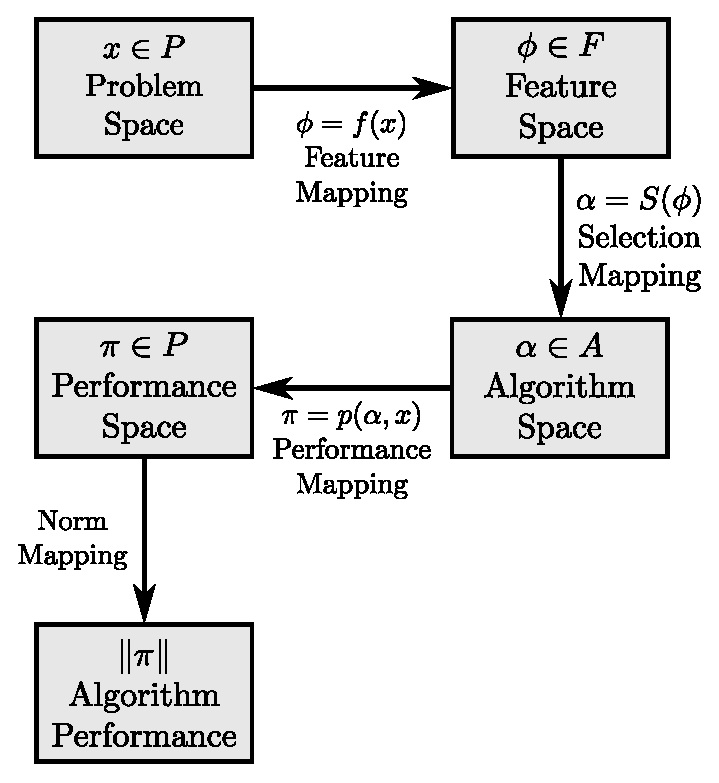
\includegraphics[width=.35\textwidth]{algorithm-selection}
    \end{center}
    \caption{Rice's framework}
    \label{fig:riceframe}
\end{figure}

\todo[inline,author=Pedro,color=cyan]{Discuss autonomous solvers}
\todo[inline,author=Pedro,color=cyan]{Discuss the choice of autotuning for
this work, given all the possibilities for solving the same problem
presented in this chapter}

\section{On-line Control}
\label{sec:oncontrol}

\subsection{Adaptive Parameter Configuration}
\label{subsec:paramadaptive}

\subsection{Credit Assignment}
\label{subsec:creditassign}

\subsection{Reinforcement Learning}
\label{subsec:reinforce}

\section{Off-line Configuration}
\label{sec:offconfig}

\subsection{Evolutionary Computing}
\label{subsec:evolcomp}

\subsection{Stochastic Local Search}
\label{subsec:searchsls}

\subsection{Machine Learning}
\label{subsec:searchml}

\section{Autotuning}
\label{chap:autotuning}

Rice's conceptual framework~\cite{rice1976algorithm} formed the foundation
of autotuners in various problem domains.  In 1997, the PHiPAC
system~\cite{bilmes1997optimizing} used code generators and search scripts to
automatically generate high performance code
for matrix multiplication. Since then, systems tackled different domains with a
diversity of strategies. Whaley \emph{et al.}~\cite{dongarra1998automatically}
introduced the ATLAS project, that optimizes dense matrix multiplication
routines. The OSKI~\cite{vuduc2005oski} library provides automatically tuned
kernels for sparse matrices. The FFTW~\cite{frigo1998fftw} library provides
tuned C subroutines for computing the Discrete Fourier Transform.
Periscope~\cite{gerndt2010automatic} is a distributed online autotuner for
parallel systems and single-node performance.

\begin{table}[htpb]
    \centering
    \begin{tabular}{@{}lll@{}}
        \toprule
        System & Domain & Technique \\ \midrule
        OSKI~\cite{vuduc2005oski} & Sparse Linear Algebra & Heuristic + Exhaustive \\
        LGen~\cite{spampinato2014basic} & Small-scale Linear Algebra & Exhaustive + Random \\
        ATLAS~\cite{dongarra1998automatically} & Dense Linear Algebra & Exhaustive \\
        INSIEME~\cite{jordan2012multi} & Compiler & Genetic Algorithm \\
        Petabricks~\cite{ansel2009petabricks} & Domain-Agnostic & Genetic Algorithm\\
        TANGRAM~\cite{chang2016efficient} & Heterogeneous Architectures & Breadth-First Search + Pruning \\
        SPIRAL~\cite{puschel2005spiral} & DSP Algorithms & Pareto Active Learning \\
        GCC Milepost~\cite{fursin2011milepost} & Compiler & Central DB + Machine Learning \\
        Apollo~\cite{beckingsale2017apollo} & GPU kernels & Decision Trees \\
        Active Harmony~\cite{tapus2002active} & Runtime & Nelder-Mead \\
        MASE-BDI~\cite{coelho2016mase} & Environmental Land Change & Distributed Active Harmony~\cite{tapus2002active} \\
        ParamILS~\cite{hutter2009paramils} & Domain-Agnostic & Stochastic Local Search \\
        CLTune~\cite{nugteren2015cltune} & OpenCL kernels & Stochastic Local Search\\
        OpenTuner~\cite{ansel2014opentuner} & Domain-Agnostic & Ensemble \\
        Periscope~\cite{gerndt2017multi} & HPC Applications & Various \\
        \bottomrule
    \end{tabular}
    \caption{Selected autotuning systems, their domains and techniques}
\end{table}

\subsection{Exhaustive Search \& Heuristics}

Abdelfattah et al.~\cite{abdelfattah2016performance} present an autotuning
strategy using exhaustive evaluation of General Matrix-Matrix Multiply (GEMM)
kernel optimizations for GPUs. They later use this approach to optimize GPU
kernels for large-scale tensor contractions~\cite{abdelfattah2016high}.
Guerreiro et al.~\cite{guerreiro2015multi} use search space pruning strategies
and exhaustive evaluation to autotune CUDA GPU kernels.  Garvey et
al.~\cite{garvey2015automatic} present a strategy to autotune OpenCL GPU
kernels using machine learning, heuristics for search space partitioning and
exhaustive search.  PolyMage~\cite{mullapudi2015polymage} is a domain-specific
language and compiler for image processing pipelines. It uses heuristics and
performance models to prune the search space, which is then explored
exhaustively.  LGen~\cite{spampinato2014basic} is a compiler for small-scale
linear algebra computation that uses mathematical domain-specific languages to
optimize loops and vectorization. LGen uses exhaustive or random search to test
different optimizations.

\subsection{Genetic Algorithms}

Ziegler et al.~\cite{ziegler2016synthesis,ziegler2016scalable} present an
autotuning system for hardware synthesis parameters that uses genetic and
learning algorithms to explore the hardware design space for real industrial
chip designs from IBM.  In an effort to provide a common representation of
multiple parallel programming models, the INSIEME compiler
project~\cite{jordan2012multi} implements abstractions for OpenMP, MPI and
OpenCL, and generates optimized parallel code for heterogeneous multi-core
architectures.

\subsection{Machine Learning}

Tartara and Reghizzi~\cite{tartara2012parallel} use the MapReduce programming
model to improve the performance of machine learning algorithms in the
PetaBricks compiler. Later they presented a machine learning
algorithm~\cite{tartara2013continuous} that learns compiler heuristics using
data gathered after every compilation.  Ngoko et al.~\cite{ngoko2016automatic}
introduce an autotuning system for $\NP$-hard problems that uses distributed
measurements of configurations and machine learning algorithms aided by
randomization, clustering and set intersection solvers.  Luo et
al.~\cite{luo2015fast} present a framework for stencil computations that uses
Optimal-Solution Spaces, input feature extraction and machine learning.
Mametjanov et al.~\cite{mametjanov2015autotuning} present an autotuning
approach that uses machine learning and selective sampling of the search space
to optimize FPGA hardware design parameters for performance and power.  Hou et
al.~\cite{hou2017auto} present an autotuning framework that uses decision trees
to optimize the sparse matrix-vector multiply kernel for multi and many-core
processors.  Apollo~\cite{beckingsale2017apollo} is an autotuning framework for
input-dependent kernels that uses a decision tree classifier that provides
optimizations that can be selected during runtime.

\subsection{Model-aided}

TuningGenie~\cite{ivanenko2014method} presents an autotuning framework that
uses code annotations and an analytical model for generating autotuners for
parallel programs.  Falsch and Elster~\cite{falch2017machine} build performance
models for OpenCL applications in different target architectures using machine
learning.  A statistical model learned and later used to pick promising
configurations for testing.  Balaprakash et al.~\cite{balaprakash2016automomml}
introduce a framework that uses machine learning algorithms to build models for
metrics such as performance and energy consumption, which are used for
multi-objective optimization.
Lang~\cite{lang2017data} reviews work on autotuning based on analytical
performance models, arguing that the approach is feasible.
Xu et al.~\cite{xu2016analytical} introduce an autotuning framework for
loop scheduling in GPUs that uses analytical performance models.

Shuchart et al.~\cite{schuchart2017readex} introduce the READEX (Runtime
Exploitation of Application Dynamism for Energy-efficient eXascale computing)
project and its methodology for developing tools to improve the energy
efficiency of High-Performance Computing applications.

The Periscope Tuning Framework
(PTF)~\cite{gerndt2005periscope,gerndt2010automatic,gerndt2017multi} is an
online tool for performance analysis and tuning that has a modular architecture
based on plugins.

Xu et al.~\cite{xu2017parallel} present an autotuning strategy that uses
parallel OpenTuner instances to autotune the FPGA compilation flow.  Their work
dynamically partition the search space between MPI-communicating OpenTuner
instances.

Active Harmony~\cite{tapus2002active} provides an API that enables
online autotuning of a program using a variation of the Nelder-Mead
simplex algorithm~\cite{nelder1965simplex}.

MASE-BDI~\cite{coelho2016mase} is a multi-agent system for the simulation of
environmental land change that uses the Active Harmony
API~\cite{tapus2002active} and search algorithms to autotune its parameters.
Several simulator configurations are executed in parallel and communicate their
results to a tuning manager using MPI.

Jayasena et al.~\cite{jayasena2015auto} use OpenTuner to implement an autotuner
for a Java Virtual Machine implementation.

CLTune~\cite{nugteren2015cltune} is an autotuning framework for OpenCL kernels
that uses search algorithms such as simulated annealing and particle swarm
optimization.

\subsection{Multiple Techniques}

Some systems provide generic tools that enable the implementation of autotuners
in various domains.  Petabricks~\cite{ansel2009petabricks} is a language and
compiler that enables the expression of program implementation search spaces at
language level.  OpenTuner~\cite{ansel2014opentuner} is a domain-agnostic
autotuning framework that provides ensembles of search techniques for
user-defined program configurations.  The ParamILS
framework~\cite{hutter2009paramils} applies stochastic local search methods for
algorithm configuration and parameter tuning. Bosboom \emph{et al.} and Eliahu
use OpenTuner to implement a domain specific language for data-flow
programming~\cite{bosboom2014streamjit} and a framework for recursive parallel
algorithm optimization~\cite{eliahu2015frpa}.
TANGRAM~\cite{chang2015tangram,chang2016efficient} is a kernel synthesis
framework for different architecture hierarchies.  It uses composition rules
and breadth-first search to prune and explore the design space.  Takizawa et
al.~\cite{takizawa2017customizable} use OpenTuner~\cite{ansel2014opentuner} and
Xevolver~\cite{takizawa2014xevolver}, a code transformation framework, to
enable the autotuning of code transformations in applications that were not
implemented for autotuning. They present an autotuning ``scenario template''
that uses compiler directives to inform the autotuner.
Williams~\cite{williams2009optimization} present optimization strategies for
the sparse matrix-vector multiply kernel in multi-core processors.  Williams et
al.~\cite{williams2009roofline} also present Roofline, a visual performance
model for parallel hardware and software that helps in the optimization of
floating-point computations.

\subsection{OpenTuner}
\label{sec:opentuner}
\todo[inline,author=Pedro,color=cyan]{Discuss OpenTuner's limitations and shortcomings.}

\subsubsection{Context}
\label{sec:context}

\subsubsection{Software Architecture}
\label{sec:arch}

\subsubsection{Parallel and Distributed Programming in OpenTuner}
\label{sec:opentuner-parallel}
\todo[inline,author=Pedro,color=cyan]{Discuss the difficulties and
explain why they motivated the new Julia code.}

\subsection{Search Techniques}
\label{sec:techniques}

\subsubsection{Numerical Methods}
\label{subsec:num}

\subsubsection{Evolutionary Computation}
\label{subsec:tuninevolcomp}

\subsubsection{Stochastic Local Search}
\label{subsec:tuningsls}

\subsubsection{Machine Learning}
\label{subsec:tuningml}

\subsection{Benchmarks}
\label{sec:benchmarks}

\subsubsection{Solvers of NP-Complete Problems}
\label{subsec:np}

\subsubsection{Algorithm Selection and Configuration}
\label{subsec:algsel}

\subsubsection{Compiler Configuration}
\label{subsec:compilerconfig}

\subsubsection{Measurement Time}
\label{subsec:measure}

\chapter{Autotuning}
\label{chap:autotuning}

\section{OpenTuner}
\label{sec:opentuner}

\subsection{Context}
\label{subsec:context}

\subsection{Software Architecture}
\label{subsec:arch}

\section{Search Techniques}
\label{sec:techniques}

\subsection{Numerical Methods}
\label{subsec:num}

\subsection{Evolutionary Computation}
\label{subsec:tuninevolcomp}

\subsection{Stochastic Local Search}
\label{subsec:tuningsls}

\subsection{Machine Learning}
\label{subsec:tuningml}

\section{Benchmarks}
\label{sec:benchmarks}

\subsection{Solvers of NP-Complete Problems}
\label{subsec:np}

\subsection{Algorithm Selection and Configuration}
\label{subsec:algsel}

\subsection{Compiler Configuration}
\label{subsec:compilerconfig}

\subsection{Measurement Time}
\label{subsec:measure}

\chapter{Case Studies}
\label{chap:usecases}

\chapter[NODAL: an Open Distributed Autotuning Library]{NODAL: \\ an Open Distributed Autotuning Library}
\label{chap:julia}

This chapter presents NODAL, a domain-agnostic autotuning library written in
the Julia language, and
available~\footnote{\url{https://github.com/phrb/NODAL.jl} [Accessed in
17/10/2017]} under the MIT license.  NODAL has had continuous integration from
the start of the project, has 96\% of the relevant lines covered by unit tests
and an online documentation. NODAL's architecture and approach to
domain-agnostic autotuning is inspired by the OpenTuner
framework~\cite{ansel2014opentuner}. Autotuners using NODAL must define a
search space using the library's parameter types, and a cost function that
generates a program configuration and measures a performance metric.

The main contribution of NODAL is providing the capability of implementing
parallel and distributed search and measurement in autotuners for different
problem domains. NODAL's language selection, software architecture, and
execution flow were intended to solve the problems identified in the OpenTuner
framework, presented in section~\ref{sec:opentuner-parallel}.

NODAL is implemented in Julia, a high-level and high-performance language.
Julia programs are not limited by a Global Interpreter Lock, and are able to
leverage multi-core architectures and distributed computing resources.
Section~\ref{sec:julia} describes the Julia language and its parallel and
distributed programming model.

The search and measurement execution flows in NODAL are not centrally managed.
Each technique is able to request measurements and update its algorithm
independently. Multiple techniques can run in parallel in the same machine, or
distributed in multiple machines.  Techniques do not share global results and
can explore different regions of the search space.
Section~\ref{sec:nodal-arch} presents the current NODAL architecture, a
simplified call graph, and the improvements we have planned.
Section~\ref{sec:nodal-components} presents a more detailed view of each search
and measurement component.  Section~\ref{sec:nodal-examples} presents two
autotuners implemented using NODAL.

\section{The Julia Language}
\label{sec:julia}

Julia~\cite{bezanson2012julia,bezanson2014julia} is a dynamic programming
language, providing a high-level syntax and programming model.  Despite that,
Julia has performance comparable to widely used statically typed, low-level
languages. The time benchmarks~\footnote{Obtained from
\url{https://julialang.org/benchmarks/} [Accessed in 17/10/2017]} shown in
Figure~\ref{fig:julia_benchmarks} compare Julia's performance with other
high-level dynamic programming languages, using the performance in the C
language as a baseline.

\begin{figure}[htpb]
    \centering
    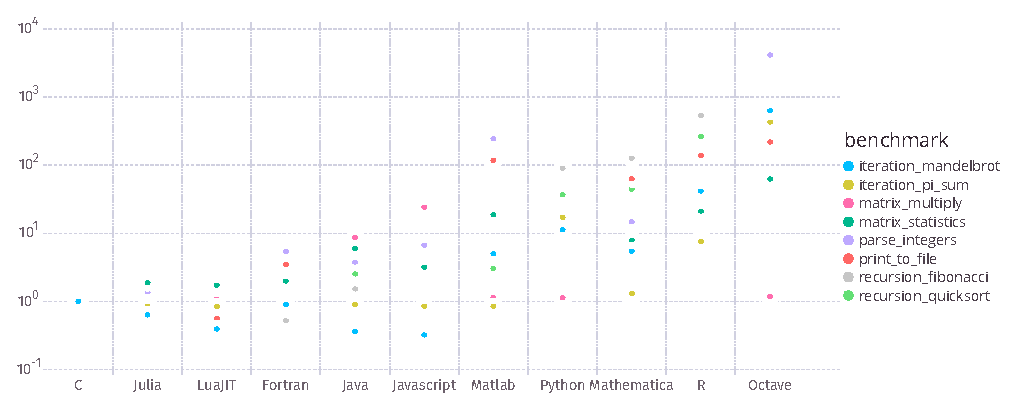
\includegraphics[width=.95\textwidth]{julia_benchmarks}
    \caption{Time benchmarks, relative to C, for various high-level languages}
    \label{fig:julia_benchmarks}
\end{figure}

The Julia developer community~\footnote{\url{https://github.com/JuliaLang/julia} [Accessed in
17/10/2017]} is very active, both in improving the standard library
and in developing separate packages, with over 1500 packages registered
in the language's official
repositories~\footnote{\url{https://pkg.julialang.org/} [Accessed in
17/10/2017]}, including NODAL.

Julia's high-performance, for a dynamic programming language, is attributed to
its type-inferred, Just-In-Time (JIT) compilation. Although a Julia program
can be written without type specifications, annotating variables with static
types is essential for performance.

\subsection{Parallel and Distributed Programming}
\label{sec:parallel-julia}

Julia's parallel and distributed programming model is based on message-passing
between processes. Each process has its own ID integer, and can run in a
separate processor core or machine. A Julia program does not manage multiple
processes, and is instead able to communicate using remote calls and
references, and data passed through channels.

Processes are launched and managed by cluster managers, which provide data
transport via TCP/IP in the built-in implementation. Cluster managers are also
able to manage the topology of the process network. NODAL currently uses the
built-in cluster manager, but studying the impact of different process
topologies might provide insight into improving NODAL's performance in
different distributed computing settings.

\subsubsection{Remote Calls \& References}

In Julia, a \textit{remote call} is a function call that is computed in a
different process. Remote calls can be made with the \texttt{remotecall}
function, or with macros from the \texttt{@spawn} family. The
\texttt{remotecall} function receives a regular function \texttt{f}, a process
ID, and the arguments to be passed to \texttt{f}. The \texttt{@spawn} macro
receives an expression, which can be a regular function call or any valid Julia
expression, and launches it in the next available Julia process.

Remote calls return immediately after launching the computation. The
results can be obtained using the \textit{remote reference} returned
by remote calls. Remote references are objects that reference data
stored in other processes, and can be of type \texttt{Future} or
\texttt{RemoteChannel}.

Figure~\ref{fig:remotecall_example} shows a code snippet that illustrates how
to use the \texttt{remotecall} function and the \texttt{@spawnat} macro. The
\texttt{@spawnat} macro receives as argument the target process in which to
launch the computation, in addition to a Julia expression. The Julia
interpreter can be launched with the \texttt{-p} argument, which receives an
integer and launches the correspondent number of Julia processes.

The code snippet in Figure~\ref{fig:remotecall_example} shows a remote call to
the \texttt{rand} function, to be launched in the process with ID 2. The other
arguments specify the 2 by 2 matrix that \texttt{rand} will fill with random
numbers. After this remote call, the computation has been launched in a remote
process, and a \texttt{Future} is returned. The interpreter does not wait for
the computation to finish and waits for new input.

\begin{figure}[htpb]
    \begin{minipage}{\linewidth}
    \begin{lstlisting}[language=C, basicstyle=\ttfamily\scriptsize,
        numbers=left,
        frame=no, showspaces=false, showstringspaces=false,
        numberstyle=\scriptsize,
        xleftmargin=1.5cm,
        keywords={%
            @spawnat, remotecall, Nullable, Any,
            fetch, Future, Array, Float64, julia%
        },
        otherkeywords={::, \&, \*, +, -, /, [, ], >, <}
    ]
% ./julia -p 2

julia> r = remotecall(rand, 2, 2, 2)
Future(2, 1, 4, Nullable{Any}())

julia> s = @spawnat 2 1 .+ fetch(r)
Future(2, 1, 5, Nullable{Any}())

julia> fetch(s)
2x2 Array{Float64,2}:
 1.18526  1.50912
 1.16296  1.60607
    \end{lstlisting}
    \end{minipage}
    \caption{Using Julia's \texttt{remotecall} function and the \texttt{@spawnat} macro}
    \label{fig:remotecall_example}
\end{figure}

The call to the \texttt{@spawnat} macro in line 6 of
Figure~\ref{fig:remotecall_example} calls the \texttt{fetch} function. This
function receives a \texttt{Future} and blocks until the result is computed by
the remote process. The \texttt{.+} syntax represents an operation in an array.
In this case, the operation is summing 1 to every element of the matrix
returned by \texttt{fetch(r)}. The \texttt{@spawnat} macro also returns a
\texttt{Future}.  Finally, the call to \texttt{fetch} in line 9 of
Figure~\ref{fig:remotecall_example} gets the final value computed by the two
remote calls. The \texttt{remotecall\_fetch} function is a more efficient way
of launching a computation in a remote process and immediately asking for the
results, if there is no computation that can be performed while the process
waits.

A \texttt{Future} caches the remotely computed value after the first call,
and returns it without process communication in subsequent calls. A process
can only write once to a \texttt{Future}. If a more extended communication
is required, the programmer needs to use remote channels.

\subsubsection{Remote Channels}

Figure~\ref{fig:remotechannel_example} shows a more complex parallel and
distributed programming example using remote channels to manage a worker pool
that performs arbitrary jobs. Remote channels are created in a specific
process, but any process with a reference to a remote channel is able to write
values to it using the \texttt{put!} function, and to read values from it using
the \texttt{take!} function. In remote channels from the standard library,
\texttt{put!} blocks until there is space in the channel and \texttt{take!}
blocks until there is a data object in the channel that can be taken, and
removing it from the channel when the call completes.

\begin{figure}[htpb]
    \begin{minipage}{\linewidth}
    \begin{lstlisting}[language=C, basicstyle=\ttfamily\scriptsize,
        numbers=left,
        frame=no, showspaces=false, showstringspaces=false,
        numberstyle=\scriptsize,
        xleftmargin=1.5cm,
        keywords={%
            @spawnat, remotecall, Nullable, Any,
            fetch, Future, Array, Float64, julia,
            while, true, function, end, put!,
            take!, sleep, RemoteChannel, Channel,
            Int, Tuple, const, addprocs, @schedule,
            @everywhere, for, in, myid, @async,
            remote_do, workers%
        },
        otherkeywords={::, \&, \*, +, -, /, [, ], >, <, put!, take!}
    ]
julia> addprocs(4)

julia> const jobs = RemoteChannel(()->Channel{Int}(32))

julia> const results = RemoteChannel(()->Channel{Tuple}(32))

julia> @everywhere function do_work(jobs, results) # Defines method everywhere
       while true
           job_id = take!(jobs)
           exec_time = rand()
           sleep(exec_time) # Simulates time doing work
           put!(results, (job_id, exec_time, myid()))
       end
   end

julia> function make_jobs(n)
           for i in 1:n
               put!(jobs, i)
           end
       end

julia> n = 12

julia> @schedule make_jobs(n)

julia> for p in workers()
           @async remote_do(do_work, p, jobs, results)
       end

julia> while n > 0 # print out results
           job_id, exec_time, where = take!(results)
           n = n - 1
       end
    \end{lstlisting}
    %$
    \end{minipage}
    \caption{Using Julia's \texttt{RemoteChannel}}
    \label{fig:remotechannel_example}
\end{figure}

The snippet in Figure~\ref{fig:remotechannel_example} uses other macros and
functions. The \texttt{addprocs} function adds a specific number of processes
to the worker pool. The \texttt{@everywhere} macro is used to define data, or a
function, in all available Julia processes. The \texttt{@schedule} and
\texttt{@async} macros add asynchronous expressions to the Julia scheduler.
The \texttt{remote\_do} function launches a function in a given worker or
worker pool object.

NODAL uses remote calls and references to perform measurements, and remote
channels to manage the communication between search techniques and the user
program. The following section will describe NODAL's architecture and its
parallel and distributed implementation.

\section{Software Architecture}
\label{sec:nodal-arch}

Our main concern when developing NODAL was to ensure that search techniques
were independent from each other, making and managing their own requests for
measurements. To achieve this objective we developed a software architecture
that minimizes communication between processes and does not block on requests
to channels. NODAL uses a custom non-blocking remote channel, the
\texttt{ResultChannel}. Search techniques manage their own execution flow, and
write their results to remote channels. A central control process regularly
polls those remote channels for results.

\begin{figure}[htpb]
    \centering
    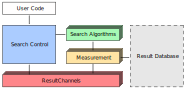
\includegraphics[width=.65\textwidth]{nodal_architecture}
    \caption{NODAL architecture, with a proposed database}
    \label{fig:nodal_architecture}
\end{figure}

Figure~\ref{fig:nodal_architecture} shows a high-level representation of
NODAL's architecture. User code that uses the library is responsible for
launching the main NODAL process, or \textit{tuning run}, and communicates with
it using remote channels. The NODAL main process is responsible for
initializing parallel and distributed search techniques using all processes
available. Each technique writes the best result it has found so far to its own
remote channel.  The main process has references for all technique remote
channels, and periodically polls them for results.  After technique
initialization there is no blocking communication between the main process and
search techniques, and no communication between search techniques.

Search techniques are responsible for generating candidate configurations for
evaluation and requesting their measurement. This is done using remote calls to
the user-defined cost function. After measurement is complete, search
techniques write the current result to their remote channel.  The non-blocking
remote channel implementation used in NODAL  is described in
section~\ref{sec:nodal-measurement}.

Figure~\ref{fig:nodal_architecture} shows a grayed out database component,
which is not yet implemented. This database will shorten the time to obtain
measurements of repeated configurations, and has the potential to be used to
train machine learning models or to give to the user knowledge about the search
space.

\subsection{Search and Measurement Call Graph}

A more detailed NODAL execution flow is presented in
Figure~\ref{fig:nodal_callgraph}. Each colored box represents a colored
component of Figure~\ref{fig:nodal_architecture}, and each smaller named box
represents a function of each component. When necessary, a number marks the
order in which functions are called.

The entry point of a NODAL application is the user code, which calls the
\texttt{optimize} function. This is the main NODAL process, and must be
launched using a remote call. The main process initializes remote search
techniques, using remote calls, by calling the
\texttt{initialize\_search\_tasks!} function. It is a non-enforced style of the
Julia language to append a ``\texttt{!}'' to functions that modify their
arguments. In this case, the modified argument is the list of remote channels
stored by the main process.  The initialization process is non-blocking, and it
returns after all techniques have been launched. The main process then enters a
loop, periodically checking for results from its remote channel references.
The \texttt{put!} and \texttt{take!} functions of \texttt{ResultChannel} are
non-blocking, so the main process always instantly gets a result from the
channel.

Initialized search techniques run their algorithms using search building
blocks, which are functions that perform some operation on the current
configuration of a search technique, measure it, and decide whether to accept
the new configuration. For example, the simulated annealing technique uses
the probabilistic improvement search building block.

\begin{figure}[htpb]
    \centering
    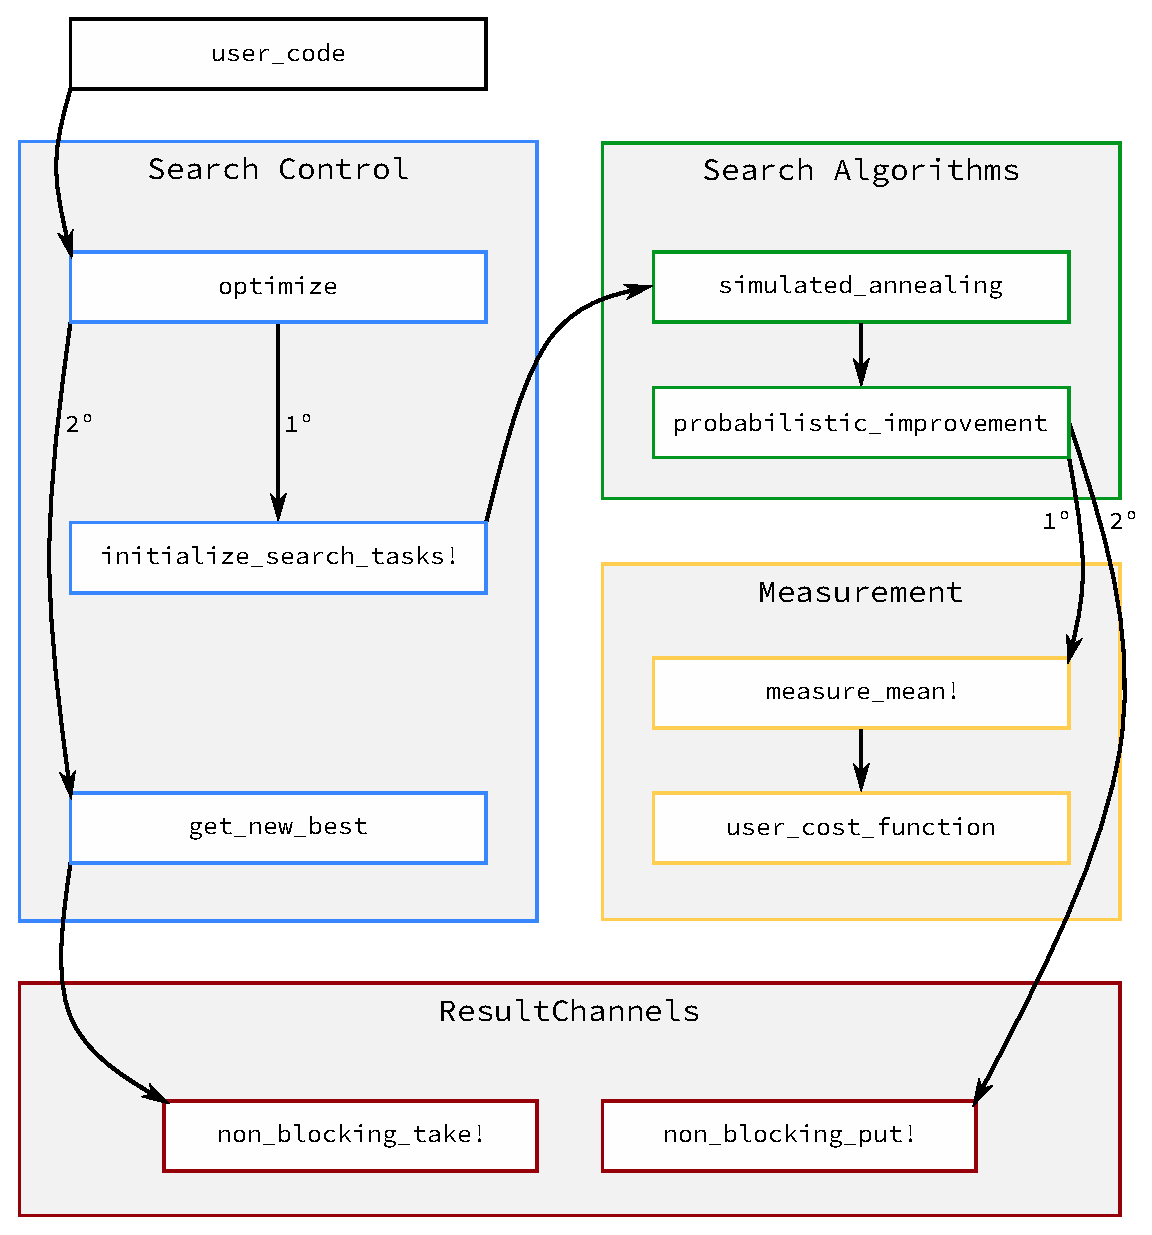
\includegraphics[width=.5\textwidth]{nodal_callgraph}
    \caption{NODAL search and measurement simplified call graph}
    \label{fig:nodal_callgraph}
\end{figure}

Search techniques request a measurement by performing remote calls to the
user-defined cost function. One way to do that is using the
\texttt{measure\_mean!} function, which perform multiple evaluations of a
function in parallel and returns the average of the measurements.  This is
useful for time measurements, for example, where fluctuations on the operating
system or system load can interfere with the results.

After a measurement is performed, a search technique can update its algorithm
and immediately request another measurement.  Search techniques do not share
their current best results with other techniques, but this was an
implementation choice and not an architecture limitation.  We intend to
implement a main process parameter that can be set by the user, and enables
global result sharing in cases where it may be beneficial. For example, the
user should be able to select which groups of techniques from the ensemble will
be allowed share their results.

\section{Search \& Measurement Components}
\label{sec:nodal-components}

This section presents in more detail the search and measurement components,
discussing available parameters, search techniques, and measurement methods.

\subsection{Search}

The search space of an autotuner implemented using NODAL is defined by a
\texttt{Configuration} object that contains a set of \texttt{Parameter}
objects. Parameters are changed by search algorithms by using operator
functions specific to each parameter type. Currently, the only operator
available in NODAL is the neighbor operator, that randomizes a parameter's
value inside a user-defined neighborhood. The ``radius'' of the neighborhood
can be changed on each call to the operator, enabling search techniques to
dynamically manipulate parameters.

\subsubsection{Parameters}

Parameters are used to define performance-impacting program variables and their
limits. They represent program configurations such as compiler flags,
enumerations of algorithms that solve a same problem, and any configurable
property of a program. Each parameter can have an initial value or left
uninitialized, in which case it will be randomized at the start of the search
process.  Table~\ref{tab:nodal-parameters} shows the parameters currently
implemented in NODAL and the planned additions.

\begin{table}[htpb]
\centering
\begin{tabular}{@{}p{.15\textwidth}p{.15\textwidth}@{}}
\toprule
\textit{Implemented} & \textit{Planned} \\ \midrule
Boolean & Logarithmic \\
Float & Exponential \\
Integer & Factorial \\
Enumeration & \\
Permutation & \\ \bottomrule
\end{tabular}
\caption{NODAL implemented and planned parameters}
\label{tab:nodal-parameters}
\end{table}

\subsubsection{Search Building Blocks}

Search building blocks are responsible for generating a new candidate
configuration and launching parallel measurements for it. Search techniques can
use one or more building blocks to implement their algorithms. Building blocks
enable users to implement parallel and distributed search techniques without
having to write parallel code in Julia or becoming familiar with NODAL
specifics. The implemented and planned building blocks at this stage of NODAL's
development comprise the necessary blocks for implementing the stochastic local
search algorithms presented by Hoos and Stützle~\cite{hoos2015stochastic}.
Other search building blocks may be necessary to implement future techniques.
Table~\ref{tab:nodal-blocks} shows the building blocks currently implemented in
NODAL and the planned additions.

\begin{table}[htpb]
\centering
\begin{tabular}{@{}p{.3\textwidth}p{.3\textwidth}@{}}
\toprule
\textit{Implemented} & \textit{Planned} \\ \midrule
First improvement & Best Improvement \\
Probabilistic Improvement & \\
Greedy Construction & \\
Random Walk & \\ \bottomrule
\end{tabular}
\caption{NODAL implemented and planned search building blocks}
\label{tab:nodal-blocks}
\end{table}

\subsubsection{Search Techniques}

The current available ensemble of search techniques in NODAL is composed of
stochastic local search techniques from the study by Hoos and
Stützle~\cite{hoos2015stochastic}.  Table~\ref{tab:nodal-techniques} present
the search techniques currently implemented in NODAL and the planned
additions.

\begin{table}[htpb]
\centering
\begin{tabular}{@{}p{.4\textwidth}p{.35\textwidth}@{}}
\toprule
\textit{Implemented} & \textit{Planned} \\ \midrule
Iterative First Improvement & Iterative Best Improvement \\
Iterative Greedy Construction & Randomized Best Improvement \\
Iterative Probabilistic Improvement & Randomized Best Improvement \\
Randomized First Improvement & Iterative Best Construction \\
Simulated Annealing & Dynamic Local Search \\
Iterated Local Search & Tabu Search \\
 & Ant Colony Optimization \\
 & Particle Swarm Optimization \\
 & Nelder-Mead \\
 & Genetic Algorithms \\ \bottomrule
\end{tabular}
\caption{NODAL implemented and planned search techniques}
\label{tab:nodal-techniques}
\end{table}

NODAL provides a simple way of creating new search techniques from building
blocks. Figure~\ref{fig:simulated_annealing} shows an implementation of the
simulated annealing search technique using the probabilistic improvement search
building block. This building block randomizes a configuration within a small
neighborhood, measures it, and accepts a worse configuration with a given
probability. This simulated annealing implementation uses a logarithmic
decreasing temperature as the probability for the probabilistic improvement
block.

Search technique functions must receive references to a \texttt{Run} object and
to a \texttt{RemoteChannel}.  The \texttt{Run} object contains the
configuration of the current tuning run, with data such as its duration,
configuration and cost function.

The search technique function must define an iteration function, which is
responsible for generating and measuring new configurations.  This function
must receive a tuning run object and return an object of type \texttt{Result}.
In NODAL, the \texttt{Result} object contains all information about a
configuration measurement, such as the iteration in which it was measured, the
measurement value and its associated configuration, and the search technique
that found it.

\begin{figure}[htpb]
    \begin{minipage}{\linewidth}
    \begin{lstlisting}[language=C, basicstyle=\ttfamily\scriptsize,
        numbers=left,
        frame=no, showspaces=false, showstringspaces=false,
        numberstyle=\scriptsize,
        xleftmargin=1.5cm,
        keywords={%
            @spawnat, remotecall, Nullable, Any,
            @fetch, Future, Array, Float64, julia,
            while, true, function, end, put!,
            take!, sleep, RemoteChannel, Channel,
            Int, Tuple, const, addprocs, @schedule,
            @everywhere, for, in, myid, @async,
            remote_do, workers, Result, Real,
            AbstractFloat, deepcopy, rand, exp, true,
            Function, false, Run, return%
        },
        otherkeywords={::, \&, \*, +, -, /, [, ], >, <, put!, take!, neighbor!,
                       update!}
    ]
function simulated_annealing(tuning_run::Run,
                             channel::RemoteChannel;
                             temperature::Function = log_temperature)
    iteration = 1

    function iterate(tuning_run::Run)
        p          = temperature(iteration)
        iteration += 1
        return probabilistic_improvement(tuning_run, threshold = p)
    end

    technique(tuning_run,
              channel,
              iterate,
              name = "Simulated Annealing")
end
    \end{lstlisting}
    %$
    \end{minipage}
    \caption{The simulated annealing search technique}
    \label{fig:simulated_annealing}
\end{figure}

The last operation of a search technique function definition must be to call
the \texttt{technique} function, passing to it the current tuning run object,
the remote channel and the iteration function. The search technique can also
define a name for itself, which will be used to tag the results it finds.

Each search technique runs in a separate Julia process, in its own
memory space. The only communication it has with the main process
is via remote result channels. We intend to add more communication
channels for configuring whether a technique should share its results
and for dynamically redistributing techniques in the search space.

\subsection{Measurement}
\label{sec:nodal-measurement}

Measurements can also be performed in different processes.
Figure~\ref{fig:nodal-measurement} shows the two measurement functions
implemented in NODAL. The \texttt{measure\_mean!} function receives a tuning
run object and a target configuration, and in this context, a configuration
means a specific point in the search space. Then, the measurement function
launches parallel measurements of the user-defined cost function with the
received configuration. The number of measurements of the cost function is
controlled by the user, and is useful for measurements that are influenced by
system fluctuations, such as execution time measurements.

\begin{figure}[htpb]
    \begin{minipage}{\linewidth}
    \begin{lstlisting}[language=C, basicstyle=\ttfamily\scriptsize,
        numbers=left,
        frame=no, showspaces=false, showstringspaces=false,
        numberstyle=\scriptsize,
        xleftmargin=1.5cm,
        keywords={%
            @spawnat, remotecall, Nullable, Any,
            @fetch, Future, Array, Float64, julia,
            while, true, function, end, put!,
            take!, sleep, RemoteChannel, Channel,
            Int, Tuple, const, addprocs, @schedule,
            @everywhere, for, in, myid, @async,
            remote_do, workers, Result, Real,
            AbstractFloat, deepcopy, rand, exp, true,
            Function, false, Run, Array, Configuration,
            pmap, mean, return%
        },
        otherkeywords={::, \&, \*, +, -, /, [, ], >, <, put!, take!, neighbor!,
                       update!}
    ]
function measure_mean!(tuning_run::Run, x::Configuration)
    configurations = Array{Configuration}(tuning_run.cost_evaluations)
    fill!(configurations, deepcopy(x))

    pmap_cost(x::Configuration) = tuning_run.cost(x, tuning_run.cost_arguments)
    results = pmap(pmap_cost, configurations)

    for i = 1:tuning_run.cost_evaluations
        tuning_run.cost_values[i] = results[i]
    end

    mean(results)
end

function sequential_measure_mean!(tuning_run::Run, x::Configuration)
    for i = 1:tuning_run.cost_evaluations
        tuning_run.cost_values[i] = tuning_run.cost(x, tuning_run.cost_arguments)
    end
    mean(tuning_run.cost_values)
end
    \end{lstlisting}
    %$
    \end{minipage}
    \caption{Parallel and distributed measurement functions}
    \label{fig:nodal-measurement}
\end{figure}

The \texttt{sequential\_measure\_mean!} function is useful when all Julia
processes are running on the same physical machine and the measured
configuration consumes all the machine's resources, or suffers
interference from other parallel measurements of the same target program. An
example of this case in the autotuning of GPU compiler flags, where more than
one of the same GPU is not always available and only one application at a time
can effectively use all the GPU's computational power.

\subsubsection{Result Remote Channels}

Figure~\ref{fig:nodal-resultchannel} shows the implementation of the
\texttt{ResultChannel} type, responsible for the communication of measurement
results between search techniques, search building blocks, and the main
process.

Our implementation of the \texttt{put!} function adds a method to the standard
library's \texttt{put!}, making sure that the result channel only updates its
value if the new value is better than the last.  Julia uses multiple-dispatch
to determine which function will be used for every argument set passed in a
function call.  When a programmer writes a function with the name of
an existing function, but with different arguments, Julia registers this new
function as a \textit{method} of the original function. Julia always
picks the most specific version of a function for its arguments, so our
\texttt{put!} implementation will always be used for objects of type
\texttt{ResultChannel}.

\begin{figure}[htpb]
    \begin{minipage}{\linewidth}
    \begin{lstlisting}[language=C, basicstyle=\ttfamily\scriptsize,
        numbers=left,
        frame=no, showspaces=false, showstringspaces=false,
        numberstyle=\scriptsize,
        xleftmargin=1.5cm,
        keywords={%
            @spawnat, remotecall, Nullable, Any,
            @fetch, Future, Array, Float64, julia,
            while, true, function, end, put!,
            take!, sleep, RemoteChannel, Channel,
            Int, Tuple, const, addprocs, @schedule,
            @everywhere, for, in, myid, @async,
            remote_do, workers, Result, Real,
            AbstractFloat, deepcopy, rand, exp, true,
            Function, false, Run, mutable, struct,
            ResultChannel, AbstractChannel, return%
        },
        otherkeywords={::, \&, \*, +, -, /, [, ], >, <, put!, take!, neighbor!,
                       update!}
    ]
mutable struct ResultChannel <: AbstractChannel
    current_result::Result
    ResultChannel(result::Result) = new(result)
end

function put!(channel::ResultChannel, result::Result)
    if result.cost_minimum < channel.current_result.cost_minimum
        channel.current_result = result
    end
    channel
end

function take!(channel::ResultChannel)
    fetch(channel)
end

function fetch(channel::ResultChannel)
    channel.current_result
end
    \end{lstlisting}
    %$
    \end{minipage}
    \caption{\texttt{ResultChannel} Implementation}
    \label{fig:nodal-resultchannel}
\end{figure}

The \texttt{take!} function also a adds a method to the standard library's
\texttt{take!}. Our implementation calls the \texttt{fetch} function,
with is also a method of \texttt{fetch} from the standard library. Our
version of \texttt{take!} immediately returns a reference to the
current value in the channel.

The \texttt{ResultChannel} constructor, shown in line 3 of
Figure~\ref{fig:nodal-resultchannel}, requires an initial result to be put into
the channel. This last implementation detail, combined with the \texttt{put!}
and \texttt{take!} methods, guarantees that there will always be a valid result
in the channel, and that only better results will be reported to the main
process.

\section{Examples}
\label{sec:nodal-examples}

This section presents two examples of using NODAL to implement
autotuners.

\subsection{The Rosenbrock Function}
\label{sec:nodal-rosenbrock}

The following is a very simple example, and you can find the source code for
its latest version in the GitHub
repository~\footnote{\url{https://github.com/phrb/NODAL.jl/blob/master/examples/rosenbrock/rosenbrock.jl}
[Accessed in 18/10/2017]}.
We will optimize the Rosenbrock function~\cite{rosenbrock1960automatic}, a
performance test function for optimization algorithms defined in
Equation~\ref{eq:rosenbrock}.  The Rosenbrock function has a global minimum
$f(a, a^{2}) = f(1,1) = 0$.  Note that the Rosenbrock function is not a
good empirical autotuning example, since its evaluation time is very short, but
it is a good initial problem.

\begin{equation}
    f(x, y) = (a - x)^{2} + b(y - x^{2})^{2}, \; \text{where} \; a = 1, \; b = 100
    \label{eq:rosenbrock}
\end{equation}

To optimize the Rosenbrock function using NODAL, the first step is defining a
\texttt{Configuration} that represents the arguments to be tuned. We also have
to create and configure a tuning run.  First, we will define the cost function
as shown in Figure~\ref{fig:nodal-cost}.

\begin{figure}[htpb]
    \begin{minipage}{\linewidth}
    \begin{lstlisting}[language=C, basicstyle=\ttfamily\scriptsize,
        numbers=left,
        frame=no, showspaces=false, showstringspaces=false,
        numberstyle=\scriptsize,
        xleftmargin=1.5cm,
        keywords={%
            @spawnat, remotecall, Nullable, Any,
            @fetch, Future, Array, Float64, julia,
            while, true, function, end, put!,
            take!, sleep, RemoteChannel, Channel,
            Int, Tuple, const, addprocs, @schedule,
            @everywhere, for, in, myid, @async,
            remote_do, workers, Result, Real,
            AbstractFloat, deepcopy, rand, exp, true,
            Function, false, Run, mutable, struct,
            begin, Configuration, Dict, Symbol, using, import,
            ResultChannel, AbstractChannel, return%
        },
        otherkeywords={::, \&, \*, +, -, /, [, ], >, <, put!, take!, neighbor!,
                       update!}
    ]
addprocs()

import NODAL

@everywhere begin
    using NODAL
    function rosenbrock(x::Configuration, parameters::Dict{Symbol, Any})
        return (1.0 - x["i0"].value)^2 + 100.0 * (x["i1"].value - x["i0"].value^2)^2
    end
end
    \end{lstlisting}
    \end{minipage}
    \caption{Initializing NODAL and defining a cost function}
    \label{fig:nodal-cost}
\end{figure}

The \texttt{addprocs} function adds the default number of Julia workers, one
per processing core, to the application. The \texttt{import} statement loads
NODAL in the current Julia worker, and the \texttt{@everywhere} macro defines
the \texttt{rosenbrock} function and the module in all Julia workers available.

Cost functions must accept a \texttt{Configuration} and a \texttt{Dict{Symbol,
Any}} as input. The \texttt{Configuration} is used to define the autotuner's
search space, and the parameter dictionary can store data or function
configurations.

This cost function ignores the parameter dictionary, and uses the \texttt{i0}
and \texttt{i1} parameters of the received configuration to compute a value.
There is no restriction on the names of \texttt{Configuration} parameters.

This configuration has two parameters of type \texttt{FloatParameter}, which
are \texttt{Float64} values constrained to an interval. The intervals are
$[-2.0, 2.0]$ for both parameters, and their values start at $0.0$. Since we
already used the \texttt{i0} and \texttt{i1} in the cost function, we must name
the parameters the same way. Figure~\ref{fig:nodal-configuration} shows
the configuration definition.

\begin{figure}[htpb]
    \begin{minipage}{\linewidth}
    \begin{lstlisting}[language=C, basicstyle=\ttfamily\scriptsize,
        numbers=left,
        frame=no, showspaces=false, showstringspaces=false,
        numberstyle=\scriptsize,
        xleftmargin=1.5cm,
        keywords={%
            @spawnat, remotecall, Nullable, Any,
            @fetch, Future, Array, Float64, julia,
            while, true, function, end, put!,
            take!, sleep, RemoteChannel, Channel,
            Int, Tuple, const, addprocs, @schedule,
            @everywhere, for, in, myid, @async,
            remote_do, workers, Result, Real,
            AbstractFloat, deepcopy, rand, exp, true,
            Function, false, Run, mutable, struct,
            begin, Configuration, Dict, Symbol, using, import,
            FloatParameter,
            ResultChannel, AbstractChannel, return%
        },
        otherkeywords={::, \&, \*, +, -, /, [, ], >, <, put!, take!, neighbor!,
                       update!}
    ]
configuration = Configuration([FloatParameter(-2.0, 2.0, 0.0, "i0"),
                               FloatParameter(-2.0, 2.0, 0.0, "i1")],
                               "rosenbrock_config")
    \end{lstlisting}
    \end{minipage}
    \caption{Defining a NODAL search space using a configuration}
    \label{fig:nodal-configuration}
\end{figure}

The next step is configuring a new tuning run using the \texttt{Run} type.
There are many parameters to configure, but they all have default values.
Figure~\ref{fig:nodal-tuningrun} shows the tuning run configuration for this
example.

\begin{figure}[htpb]
    \begin{minipage}{\linewidth}
    \begin{lstlisting}[language=C, basicstyle=\ttfamily\scriptsize,
        numbers=left,
        frame=no, showspaces=false, showstringspaces=false,
        numberstyle=\scriptsize,
        xleftmargin=1.5cm,
        keywords={%
            @spawnat, remotecall, Nullable, Any,
            @fetch, Future, Array, Float64, julia,
            while, true, function, end, put!,
            take!, sleep, RemoteChannel, Channel,
            Int, Tuple, const, addprocs, @schedule,
            @everywhere, for, in, myid, @async,
            remote_do, workers, Result, Real,
            AbstractFloat, deepcopy, rand, exp, true,
            Function, false, Run, mutable, struct,
            begin, Configuration, Dict, Symbol, using, import,
            FloatParameter,
            ResultChannel, AbstractChannel, return%
        },
        otherkeywords={::, \&, \*, +, -, /, [, ], >, <, put!, take!, neighbor!,
                       update!}
    ]
tuning_run = Run(cost                = rosenbrock,
                 starting_point      = configuration,
                 stopping_criterion  = elapsed_time_criterion,
                 report_after        = 10,
                 reporting_criterion = elapsed_time_reporting_criterion,
                 duration            = 60,
                 methods             = [[:simulated_annealing 1];
                                        [:iterative_first_improvement 1];
                                        [:iterated_local_search 1];
                                        [:randomized_first_improvement 1];
                                        [:iterative_probabilistic_improvement 1];
                                        [:iterative_greedy_construction 1];])
    \end{lstlisting}
    \end{minipage}
    \caption{Configuring a NODAL tuning run}
    \label{fig:nodal-tuningrun}
\end{figure}

The \texttt{methods} array defines the search methods that will be used in this
tuning run, and their respective number of instances. This example uses one
instance of every implemented search technique. The search will start at the
point defined by \texttt{starting\_point}.

The \texttt{stopping\_criterion} parameter is a function. It controls when the
autotuner will stop searching. The two default criteria implemented are
\texttt{elapsed\_time\_criterion} and \texttt{iterations\_criterion}.  The
\texttt{reporting\_criterion} parameter is also function, and it controls when
the autotuner reports the current results. The two default NODAL
implementations of reporting criteria are
\texttt{elapsed\_time\_reporting\_criterion} and
\texttt{iterations\_reporting\_criterion}.

Now we can start the autotuner using the \texttt{@spawn} macro. This macro runs
the \texttt{optimize} method, which receives a tuning run configuration and
runs the search techniques in the background. The autotuner will write its
results to the \texttt{RemoteChannel} stored in the tuning run configuration.
Figure~\ref{fig:nodal-launching} shows how to launch the autotuner.

\begin{figure}[htpb]
    \begin{minipage}{\linewidth}
    \begin{lstlisting}[language=C, basicstyle=\ttfamily\scriptsize,
        numbers=left,
        frame=no, showspaces=false, showstringspaces=false,
        numberstyle=\scriptsize,
        xleftmargin=1.5cm,
        keywords={%
            @spawnat, remotecall, Nullable, Any,
            @fetch, Future, Array, Float64, julia,
            @spawn,
            while, true, function, end, put!,
            take!, sleep, RemoteChannel, Channel,
            Int, Tuple, const, addprocs, @schedule,
            @everywhere, for, in, myid, @async,
            remote_do, workers, Result, Real,
            AbstractFloat, deepcopy, rand, exp, true,
            Function, false, Run, mutable, struct,
            begin, Configuration, Dict, Symbol, using, import,
            FloatParameter, @spawn,
            ResultChannel, AbstractChannel, return%
        },
        otherkeywords={::, \&, \*, +, -, /, [, ], >, <, put!, take!, neighbor!,
                       update!}
    ]
@spawn optimize(tuning_run)
result = take!(tuning_run.channel)
    \end{lstlisting}
    %$
    \end{minipage}
    \caption{Launching a NODAL tuning run}
    \label{fig:nodal-launching}
\end{figure}

The tuning run will use the default neighboring and perturbation methods
implemented by NODAL to find new results. User code can process the
current result at every iteration. In this example we just
print it and loop until \texttt{optimize} is done, as shown in
Figure~\ref{fig:nodal-mainloop}.

\begin{figure}[htpb]
    \begin{minipage}{\linewidth}
    \begin{lstlisting}[language=C, basicstyle=\ttfamily\scriptsize,
        numbers=left,
        frame=no, showspaces=false, showstringspaces=false,
        numberstyle=\scriptsize,
        xleftmargin=1.5cm,
        keywords={%
            @spawnat, remotecall, Nullable, Any,
            @fetch, Future, Array, Float64, julia,
            while, true, function, end, put!,
            take!, sleep, RemoteChannel, Channel,
            Int, Tuple, const, addprocs, @schedule,
            @everywhere, for, in, myid, @async,
            remote_do, workers, Result, Real,
            AbstractFloat, deepcopy, rand, exp, true,
            Function, false, Run, mutable, struct,
            begin, Configuration, Dict, Symbol, using, import,
            FloatParameter, @spawn, while,
            ResultChannel, AbstractChannel, return%
        },
        otherkeywords={::, \&, \*, +, -, /, [, ], >, <, put!, take!, neighbor!,
                       update!}
    ]
print(result)
while !result.is_final
    result = take!(tuning_run.channel)
    print(result)
end
    \end{lstlisting}
    %$
    \end{minipage}
    \caption{Main loop of a NODAL application}
    \label{fig:nodal-mainloop}
\end{figure}

Figure~\ref{fig:nodal-complete-example} shows the complete code for the NODAL
Rosenbrock autotuner.  Running the complete example we get the output shown in
Figure~\ref{fig:nodal-output}.  Note that every result reported shows the
technique that found the result and the iteration in which it was found. Since
the autotuner reports only at every 10 seconds, it is able to perform many
iterations between results.

\begin{figure}[htpb]
    \begin{minipage}{\linewidth}
    \begin{lstlisting}[language=C, basicstyle=\ttfamily\scriptsize,
        numbers=left,
        frame=no, showspaces=false, showstringspaces=false,
        numberstyle=\scriptsize,
        xleftmargin=1.5cm,
        keywords={%
            @spawnat, remotecall, Nullable, Any,
            @spawn,
            @fetch, Future, Array, Float64, julia,
            while, true, function, end, put!,
            take!, sleep, RemoteChannel, Channel,
            Int, Tuple, const, addprocs, @schedule,
            @everywhere, for, in, myid, @async,
            remote_do, workers, Result, Real,
            AbstractFloat, deepcopy, rand, exp, true,
            Function, false, Run, mutable, struct,
            begin, Configuration, Dict, Symbol, using, import,
            ResultChannel, AbstractChannel, return%
        },
        otherkeywords={::, \&, \*, +, -, /, [, ], >, <, put!, take!, neighbor!,
                       update!}
    ]
addprocs()

import StochasticSearch

@everywhere begin
    using StochasticSearch
    function rosenbrock(x::Configuration, parameters::Dict{Symbol, Any})
        return (1.0 - x["i0"].value)^2 + 100.0 * (x["i1"].value - x["i0"].value^2)^2
    end
end

configuration = Configuration([FloatParameter(-2.0, 2.0, 0.0,"i0"),
                               FloatParameter(-2.0, 2.0, 0.0,"i1")],
                               "rosenbrock_config")

tuning_run = Run(cost                = rosenbrock,
                 starting_point      = configuration,
                 stopping_criterion  = elapsed_time_criterion,
                 report_after        = 10,
                 reporting_criterion = elapsed_time_reporting_criterion,
                 duration            = 60,
                 methods             = [[:simulated_annealing 1];
                                        [:iterative_first_improvement 1];
                                        [:iterated_local_search 1];
                                        [:randomized_first_improvement 1];
                                        [:iterative_greedy_construction 1];
                                        [:iterative_probabilistic_improvement 1];])

@spawn optimize(tuning_run)
result = take!(tuning_run.channel)

print(result)
while !result.is_final
    result = take!(tuning_run.channel)
    print(result)
end
    \end{lstlisting}
    \end{minipage}
    \caption{Complete NODAL Rosenbrock autotuner}
    \label{fig:nodal-complete-example}
\end{figure}

\begin{figure}[htpb]
    \begin{minipage}{\linewidth}
    \begin{lstlisting}[language=C, basicstyle=\ttfamily\scriptsize,
        numbers=left,
        frame=no, showspaces=false, showstringspaces=false,
        numberstyle=\scriptsize,
        xleftmargin=1.5cm,
        keywords={%
            ResultChannel, AbstractChannel, return%
        },
        otherkeywords={::, \&, \*, +, -, /, [, ], >, <, put!, take!, neighbor!,
                       update!}
    ]
% julia rosenbrock.jl
[Result]
Cost              : 1.0
Found in Iteration: 1
Current Iteration : 1
Technique         : Initialize
Function Calls    : 1
  ***
[Result]
Cost              : 1.0
Found in Iteration: 1
Current Iteration : 3973
Technique         : Initialize
Function Calls    : 1
  ***
[Result]
Cost              : 0.18498399102098383
Found in Iteration: 10
Current Iteration : 52289
Technique         : Iterative First Improvement
Function Calls    : 455
  ***
[Result]
Cost              : 0.01301071782455056
Found in Iteration: 10
Current Iteration : 70282
Technique         : Randomized First Improvement
Function Calls    : 3940
  ***
[Result]
Cost              : 0.009463518035824526
Found in Iteration: 11
Current Iteration : 87723
Technique         : Randomized First Improvement
Function Calls    : 4594
  ***
[Final Result]
Cost                  : 0.009463518035824526
Found in Iteration    : 11
Current Iteration     : 104261
Technique             : Randomized First Improvement
Function Calls        : 4594
Starting Configuration:
  [Configuration]
  name      : rosenbrock_config
  parameters:
    [NumberParameter]
    name : i0
    min  : -2.000000
    max  : 2.000000
    value: 1.100740
    ***
    [NumberParameter]
    name : i1
    min  : -2.000000
    max  : 2.000000
    value: 1.216979
Minimum Configuration :
  [Configuration]
  name      : rosenbrock_config
  parameters:
    [NumberParameter]
    name : i0
    min  : -2.000000
    max  : 2.000000
    value: 0.954995
    ***
    [NumberParameter]
    name : i1
    min  : -2.000000
    max  : 2.000000
    value: 0.920639
    \end{lstlisting}
    \end{minipage}
    \caption{NODAL output for the Rosenbrock function example}
    \label{fig:nodal-output}
\end{figure}

\newpage

\subsection{A Tool for Compiler Autotuning}
\label{sec:nodal-gpu-tuner}

We implemented in NODAL an autotuner for the CUDA compiler parameters presented
in section~\ref{sec:paramSelGPU}. We presented this implementation at an USP
NVIDIA workshop, and its source code is available
online~\footnote{\url{https://github.com/phrb/NODAL.jl/tree/master/examples/nvcc-flags}
[Accessed in 18/10/2017]}.

Our idea was to start a community of NODAL users from High-Performance
Computing domains. We had positive feedback from the workshop, and were invited
to visit the \textit{Laboratório Nacional de Luz Síncrotron}, the Brazilian
Synchrotron Light Laboratory, a research institution on physics, chemistry,
material science and life sciences.  With this visit we expect to start
collaborating with them in autotuning their GPU applications.

\section{Summary}
\label{sec:concl}

In this chapter we presented NODAL, a library for parallel and distributed
autotuning written in Julia. We discussed relevant features of the Julia
language and presented NODAL's architecture, execution flow and implementation
details. We also discussed planned improvements, from adding a database
component to aid search, to implementing more search techniques and building
blocks. To illustrate the usage of the library, we presented two autotuners
using NODAL.

We plan to continue working in NODAL.  We expect that NODAL will be an ideal
platform for our study of complex search techniques applied to autotuning and
of strategies to divide the search space and share computational resources.  We
will also work toward building a community of users, which we expect will help
to validate and test NODAL in diverse autotuning domains.

\chapter{Summary}
\label{chap:final-summary}

\section{Objectives and Future Work}
\label{sec:future-work}

\section{Schedule}
\label{sec:schedule}


% cabeçalho para os apêndices
%\renewcommand{\chaptermark}[1]{\markboth{\MakeUppercase{\appendixname\ \thechapter}} {\MakeUppercase{#1}} }
%\fancyhead[RE,LO]{}
\appendix

%\chapter{Sequências}
\label{ape:sequencias}

Texto texto texto texto texto texto texto texto texto texto texto texto texto
texto texto texto texto texto texto texto texto texto texto texto texto texto
texto texto texto texto texto texto.


\singlespacing

\renewcommand{\arraystretch}{0.85}
\captionsetup{margin=1.0cm}  % correção nas margens dos captions.
%--------------------------------------------------------------------------------------
\begin{table}
\begin{center}
\begin{small}
\begin{tabular}{|c|c|c|c|c|c|c|c|c|c|c|c|c|} 
\hline
\emph{Limiar} & 
\multicolumn{3}{c|}{MGWT} & 
\multicolumn{3}{c|}{AMI} &  
\multicolumn{3}{c|}{\emph{Spectrum} de Fourier} & 
\multicolumn{3}{c|}{Características espectrais} \\
\cline{2-4} \cline{5-7} \cline{8-10} \cline{11-13} & 
\emph{Sn} & \emph{Sp} & \emph{AC} & 
\emph{Sn} & \emph{Sp} & \emph{AC} & 
\emph{Sn} & \emph{Sp} & \emph{AC} & 
\emph{Sn} & \emph{Sp} & \emph{AC}\\ \hline \hline
 1 & 1.00 & 0.16 & 0.08 & 1.00 & 0.16 & 0.08 & 1.00 & 0.16 & 0.08 & 1.00 & 0.16 & 0.08 \\
 2 & 1.00 & 0.16 & 0.09 & 1.00 & 0.16 & 0.09 & 1.00 & 0.16 & 0.09 & 1.00 & 0.16 & 0.09 \\
 2 & 1.00 & 0.16 & 0.10 & 1.00 & 0.16 & 0.10 & 1.00 & 0.16 & 0.10 & 1.00 & 0.16 & 0.10 \\
 4 & 1.00 & 0.16 & 0.10 & 1.00 & 0.16 & 0.10 & 1.00 & 0.16 & 0.10 & 1.00 & 0.16 & 0.10 \\
 5 & 1.00 & 0.16 & 0.11 & 1.00 & 0.16 & 0.11 & 1.00 & 0.16 & 0.11 & 1.00 & 0.16 & 0.11 \\
 6 & 1.00 & 0.16 & 0.12 & 1.00 & 0.16 & 0.12 & 1.00 & 0.16 & 0.12 & 1.00 & 0.16 & 0.12 \\
 7 & 1.00 & 0.17 & 0.12 & 1.00 & 0.17 & 0.12 & 1.00 & 0.17 & 0.12 & 1.00 & 0.17 & 0.13 \\
 8 & 1.00 & 0.17 & 0.13 & 1.00 & 0.17 & 0.13 & 1.00 & 0.17 & 0.13 & 1.00 & 0.17 & 0.13 \\
 9 & 1.00 & 0.17 & 0.14 & 1.00 & 0.17 & 0.14 & 1.00 & 0.17 & 0.14 & 1.00 & 0.17 & 0.14 \\
10 & 1.00 & 0.17 & 0.15 & 1.00 & 0.17 & 0.15 & 1.00 & 0.17 & 0.15 & 1.00 & 0.17 & 0.15 \\
11 & 1.00 & 0.17 & 0.15 & 1.00 & 0.17 & 0.15 & 1.00 & 0.17 & 0.15 & 1.00 & 0.17 & 0.15 \\
12 & 1.00 & 0.18 & 0.16 & 1.00 & 0.18 & 0.16 & 1.00 & 0.18 & 0.16 & 1.00 & 0.18 & 0.16 \\
13 & 1.00 & 0.18 & 0.17 & 1.00 & 0.18 & 0.17 & 1.00 & 0.18 & 0.17 & 1.00 & 0.18 & 0.17 \\
14 & 1.00 & 0.18 & 0.17 & 1.00 & 0.18 & 0.17 & 1.00 & 0.18 & 0.17 & 1.00 & 0.18 & 0.17 \\
15 & 1.00 & 0.18 & 0.18 & 1.00 & 0.18 & 0.18 & 1.00 & 0.18 & 0.18 & 1.00 & 0.18 & 0.18 \\
16 & 1.00 & 0.18 & 0.19 & 1.00 & 0.18 & 0.19 & 1.00 & 0.18 & 0.19 & 1.00 & 0.18 & 0.19 \\
17 & 1.00 & 0.19 & 0.19 & 1.00 & 0.19 & 0.19 & 1.00 & 0.19 & 0.19 & 1.00 & 0.19 & 0.19 \\
17 & 1.00 & 0.19 & 0.20 & 1.00 & 0.19 & 0.20 & 1.00 & 0.19 & 0.20 & 1.00 & 0.19 & 0.20 \\
19 & 1.00 & 0.19 & 0.21 & 1.00 & 0.19 & 0.21 & 1.00 & 0.19 & 0.21 & 1.00 & 0.19 & 0.21 \\
20 & 1.00 & 0.19 & 0.22 & 1.00 & 0.19 & 0.22 & 1.00 & 0.19 & 0.22 & 1.00 & 0.19 & 0.22 \\ \hline 
\end{tabular}
\caption{Exemplo de tabela.}
\label{tab:tab:F5}
\end{small}
\end{center}
\end{table}



% ---------------------------------------------------------------------------- %
% Bibliografia
\backmatter \singlespacing   % espaçamento simples
%\bibliographystyle{bib/plainnat-ime} % citação bibliográfica textual
\bibliographystyle{plainnat} % citação bibliográfica textual
\bibliography{bib/references}  % associado ao arquivo: 'bibliografia.bib'

% ---------------------------------------------------------------------------- %
% Índice remissivo
\index{TBP|see{periodicidade região codificante}}
\index{DSP|see{processamento digital de sinais}}
\index{STFT|see{transformada de Fourier de tempo reduzido}}
\index{DFT|see{transformada discreta de Fourier}}
\index{Fourier!transformada|see{transformada de Fourier}}

\printindex   % imprime o índice remissivo no documento

\end{document}
